% How to Draw Flowcharts in LaTeX using TikZ?
% latexdraw.com
% 30/01/2021 at 00:07

\documentclass[border=0.2cm]{standalone}

% Required packages
\usepackage{tikz}
\usetikzlibrary{shapes,positioning}

\begin{document}

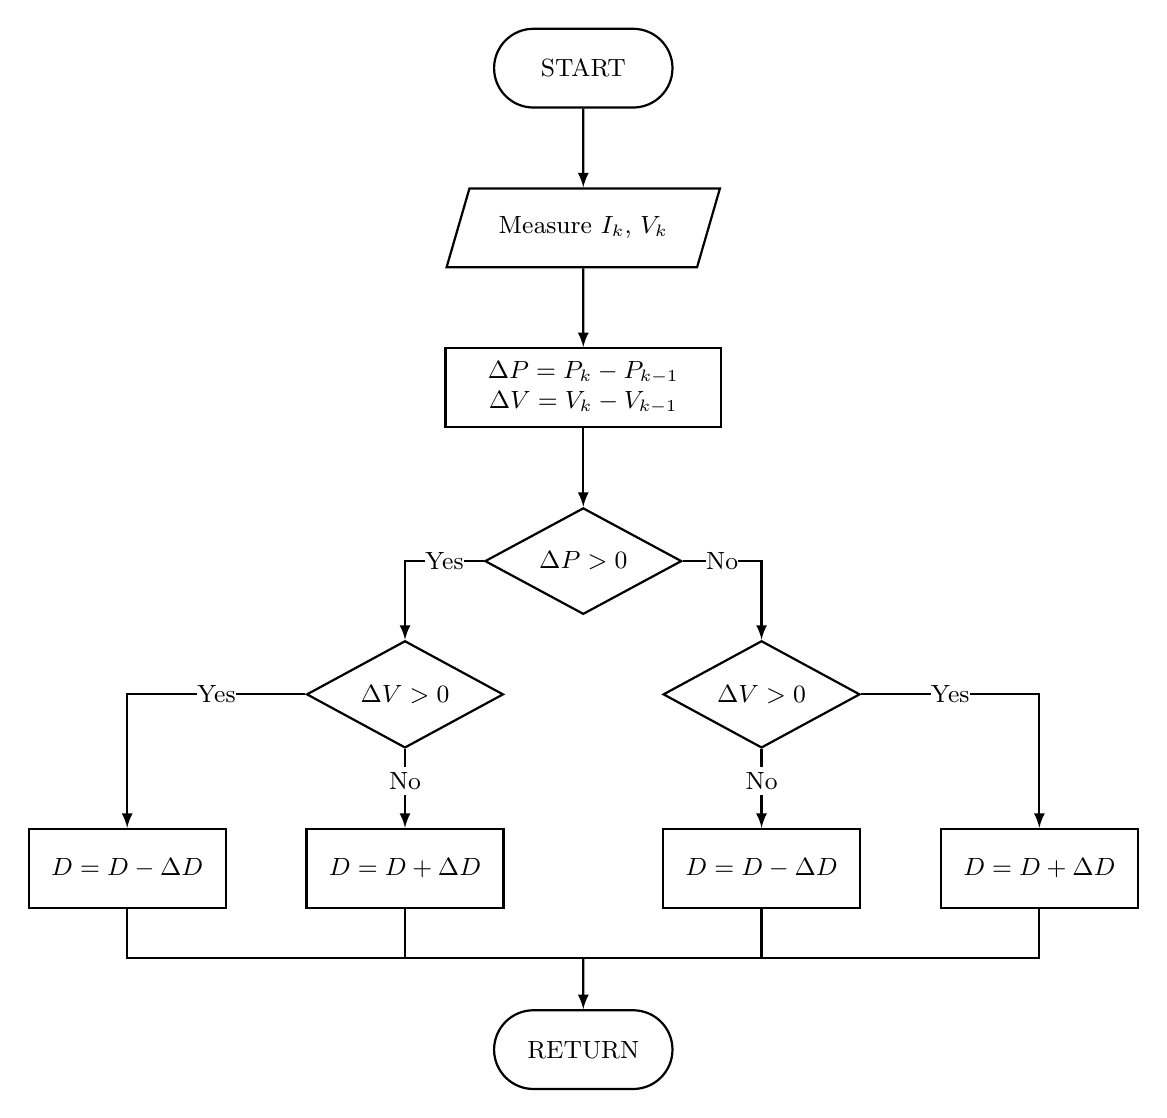
\begin{tikzpicture}[font=\small,thick]

% Start block
\node[draw,
    rounded rectangle,
    minimum width=2.5cm,
    minimum height=1cm] (block1) {START};

% Voltage and Current Measurement
\node[draw,
    trapezium, 
    trapezium left angle = 65,
    trapezium right angle = 115,
    trapezium stretches,
    below=of block1,
    minimum width=3.5cm,
    minimum height=1cm
] (block2) { Measure $I_k$, $V_k$ };

% Power and voltage variation
\node[draw,
    align=center,
    below=of block2,
    minimum width=3.5cm,
    minimum height=1cm
] (block3) { $\Delta P=P_k-P_{k-1}$ \\ $\Delta V=V_k-V_{k-1}$};

% Conditions test
\node[draw,
    diamond,
    below=of block3,
    minimum width=2.5cm,
    inner sep=0] (block4) { $\Delta P>0$};

\node[draw,
    diamond,
    below left=of block4,
    minimum width=2.5cm,
    inner sep=0] (block5) { $\Delta V>0$};

\node[draw,
    diamond,
    below right=of block4,
    minimum width=2.5cm,
    inner sep=0] (block6) { $\Delta V>0$};

% Increase and Decrease duty cycle
\node[draw,
    below=of block5,
    minimum width=2.5cm,
    minimum height=1cm] (block7) { $D=D+\Delta D$};

\node[draw,
    left=of block7,
    minimum width=2.5cm,
    minimum height=1cm] (block8) { $D=D-\Delta D$};

\node[draw,
    align=center,
    below=of block6,
    minimum width=2.5cm,
    minimum height=1cm] (block9) { $D=D-\Delta D$};

\node[draw,
    right=of block9,
    minimum width=2.5cm,
    minimum height=1cm] (block10) { $D=D+\Delta D$};

% Return block
\node[draw,
    rounded rectangle,
    below=5cm of block4,
    minimum width=2.5cm,
    minimum height=1cm,] (block11) { RETURN};

\node[coordinate,below=4.35cm of block4] (block12) {};


% Arrows
\draw[-latex] (block1) edge (block2)
    (block2) edge (block3)
    (block3) edge (block4);

\draw[-latex] (block4) -| (block5)
    node[pos=0.25,fill=white,inner sep=0]{Yes};
    
\draw[-latex] (block4) -| (block6)
    node[pos=0.25,fill=white,inner sep=0]{No};

\draw[-latex] (block5) edge node[pos=0.4,fill=white,inner sep=2pt]{No}(block7)
    (block5) -| (block8)
        node[pos=0.25,fill=white,inner sep=0]{Yes};
        
\draw[-latex] (block6) edge node[pos=0.4,fill=white,inner sep=2pt]{No}(block9)
    (block6) -| (block10)
        node[pos=0.25,fill=white,inner sep=0]{Yes};

\draw (block7) |- (block12);
\draw (block9) |- (block12);
\draw (block8) |- (block7|-block12);
\draw (block10) |- (block9|-block12);
\draw[-latex] (block12) -- (block11);

\end{tikzpicture}

\end{document}
